\section{IPS-N Raleigh}

\begin{center}
    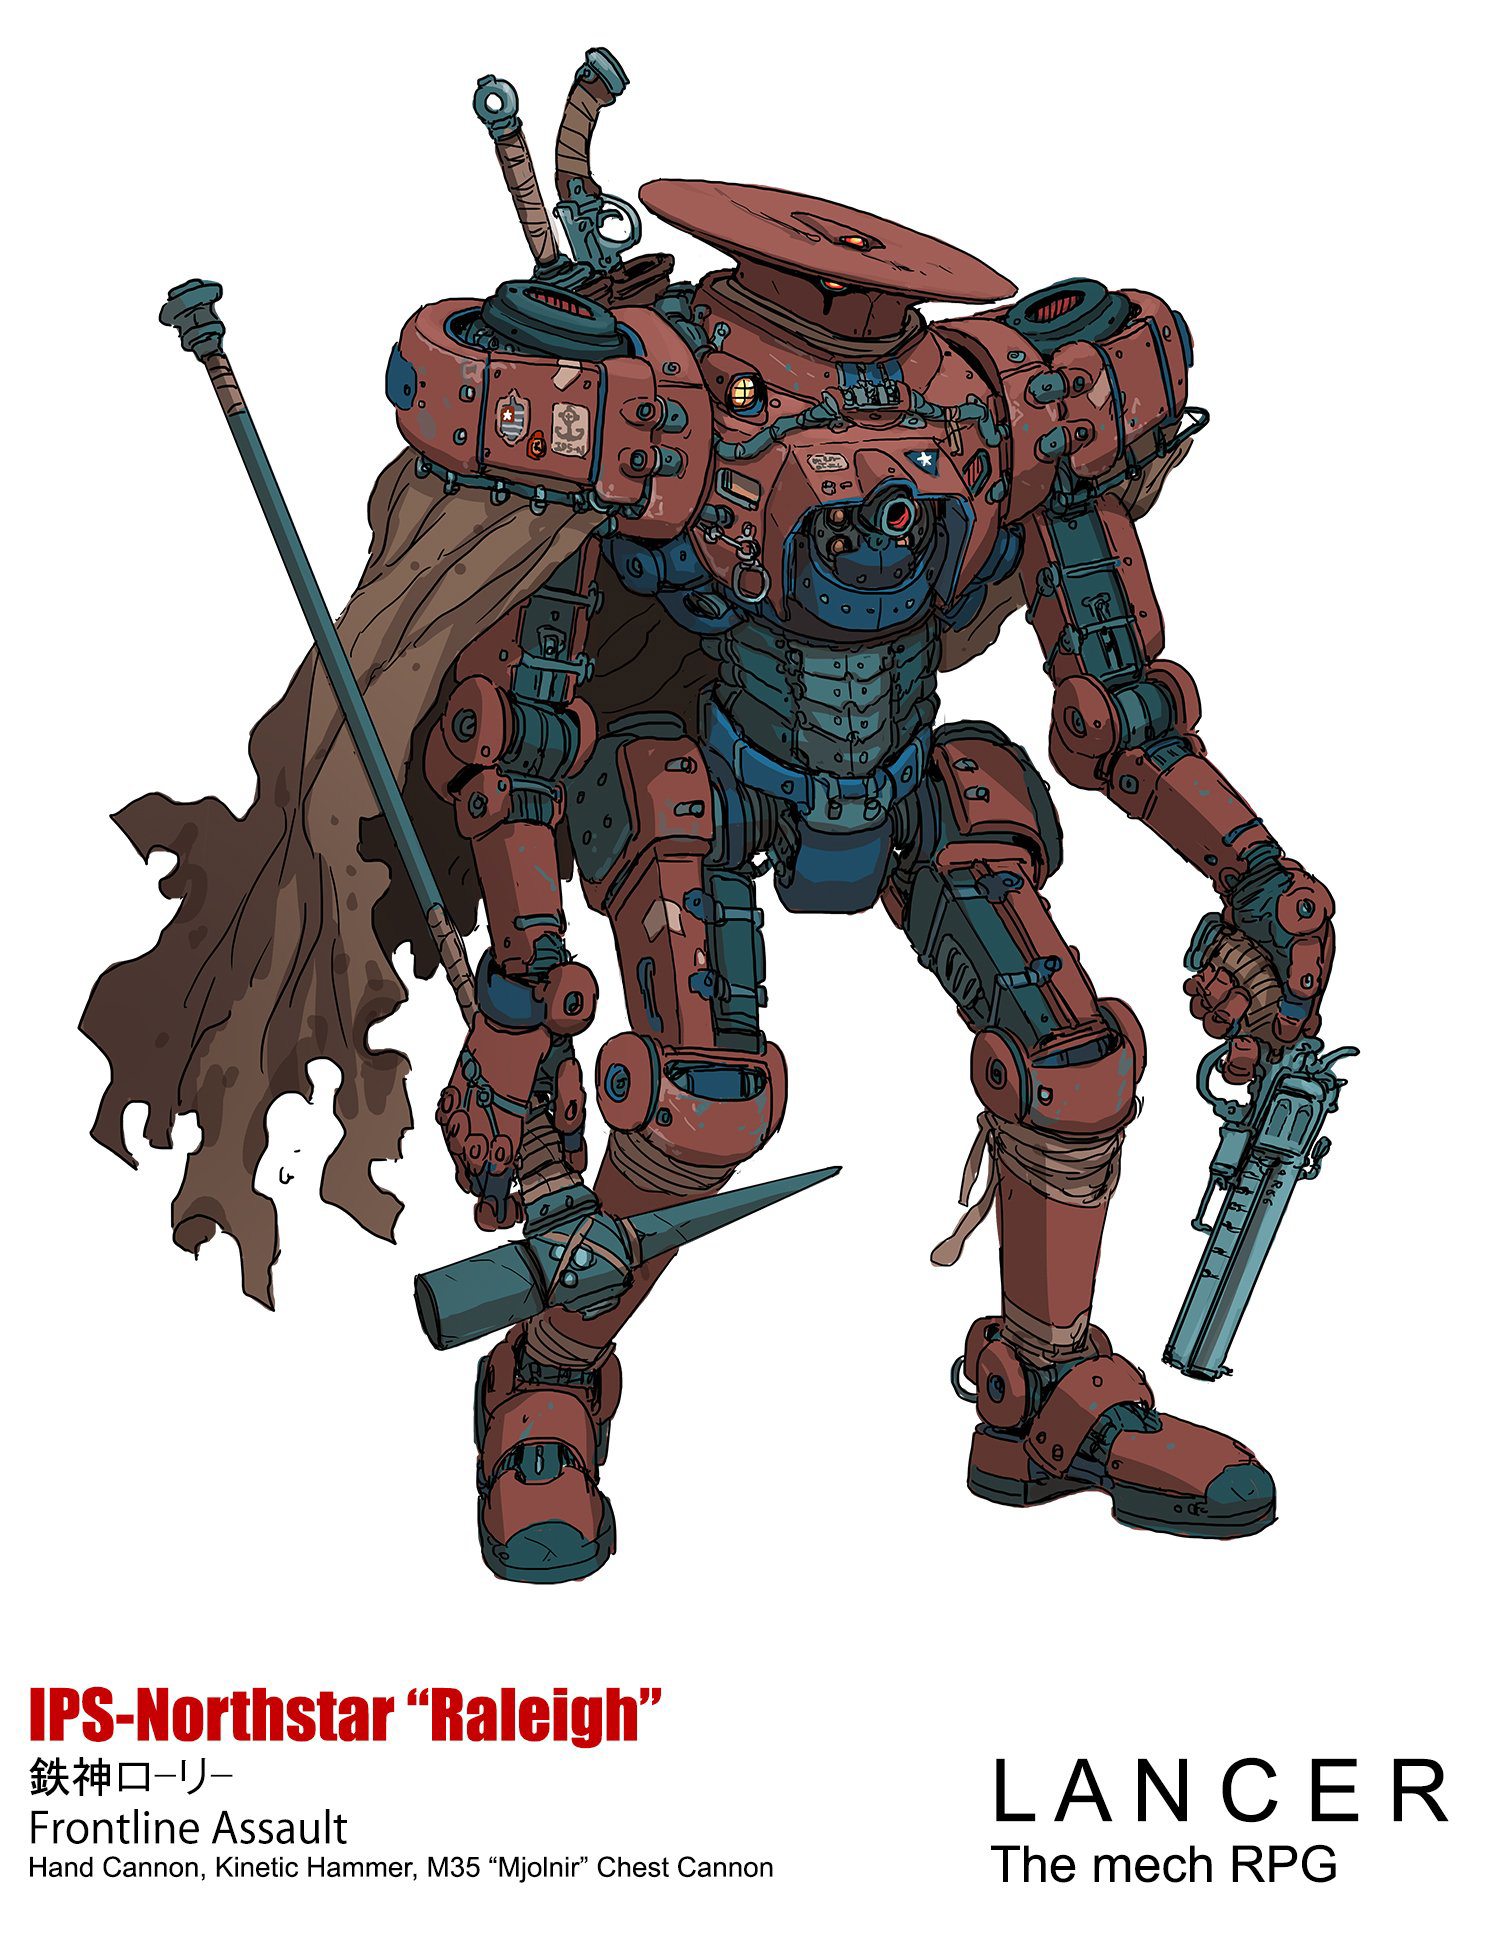
\includegraphics{Raleigh}
\end{center}

                                              IPS-N RALEIGH

The IPS-N RALEIGH, more so than any other mech in IPS-N’s core line, is meant to meet any enemy, any

where, in any combat scenario. The RALEIGH is an all-rounder build that trends towards the midrange. It is
commonly outfitted with an auxiliary hand cannon for ranged capability, a massive hammer to deal with
anything that gets close, and the iconic, chest-mounted MJOLNIR cannon.

                                                      License:

I. Hand Cannon, Breaching Charges

II. RALEIGH FRAME, ROLAND Chamber, Bolt Thrower

III. UNCLE class NHP, Kinetic Hammer





                                                    RALEIGH

  HP: 10          Evasion: 8                              Speed: 4            Heat Cap: 5         Sensors: 10

  Armor: 1        E-Defense: 8                            Size: 1             Repair Cap: 5       Tech Attack:
                                                                                                  +0

                                                      TRAITS:

  Full Metal Jacket: If the Raleigh makes no attack rolls during its turn, it can re-load all weapons with
  the loading tag at the end of its turn as a free action.

  Shielded Magazines: The Raleigh can still make ranged attacks if it is Jammed.

                                               SYSTEM POINTS: 5

                                                     MOUNTS:

  Aux/Aux                             Flex Mount                              Heavy Mount

                                                  FRAME system

                                           IPS-N M35 ‘Mjolnir’ cannon

  IPS-N’s M35 MJOLNIR cannon is a carryover from Northstar’s WATCHMAN line of defensive weapons,
  reworked for frontline combat. The MJOLNIR is a hard-mount, multi-barrel auxiliary cannon that uses
  magnetic acceleration to fire stacks of airburst projectiles at its target. It is an impulse weapon, a system
  tied to a pilot’s second-tier neural processes as dictated and coached by their partner Comp/Con or
  NHP; even in death, a pilot’s MJOLNIR will continue to identify and attack hostile targets until total
  systemic failure. For this reason, the MJOLNIR is often referred to as a deadgun, one of many such
  weapons common among CQB-oriented pilots.

  Integrated Mount:

  M35

  Main CQB

  Range 5, Threat 3

  4 kinetic damage


  Active (Requires 1 Core Power):

  Thunder God

  Protocol

  Until the end of the current challenge, if you didn’t fire your M35 on your turn, it gains 2 more rounds in
  the chamber at the end your turn (you can use a d6 to track this). It starts with 0 rounds in the chamber.
  When you next fire the weapon, it fires all chambers, for 4 damage per chamber. The M35 has six
  chambers, for a maximum of 24 damage. If 4 or more chambers are fired at once, this weapon gains
  the AP tag and any target struck must pass a hull check or be knocked prone.

Hand Cannon




The IPS-N HAND CANNON is a licensed version of GMS’s Pattern I Pistol, chambered for a heavier caliber
of round. This modification requires a change from the belt-fed system of the P1P to a magazine-based
system, limiting the number of rounds that a mech can load at a time.

Auxiliary CQB

Loading, Reliable 1

Range 5, Threat 3

1d6 damage


Breaching Charge
A breach/blast charge is simply a shaped, milspec pattern of IPS-N’s generalist/civilian blasting charge,

meant to crack asteroids. The IPS-N BB features a far more pure blend of high explosives designed to
cause massive traumatic damage to mechs and other hardened structures.

2 SP, Limited (2)
Grenade, Mine
If thrown as a quick action, the charge explodes on impact. If planted as a mine, it can be
detonated as another quick action by whoever planted it (or detonates normally when a target
moves adjacent). The charge deals 2d6 Energy damage to targets in a burst 1 area around the
charge. Targets can pass an agility check to reduce this damage by half. Against objects, this
charge does 10 AP kinetic damage.

ROLAND Chamber
Packed into sealed, self-contained cylinders, IPS-N’s ROLAND rounds are heavy shells purpose-built for
any kinetic weapon that can accept cylindrical magazines. Packed with a non-O2 dependent accelerant,
ROLAND Chambers can be used to reliably send air-or-impact burst shells downrange.

For use in outdoor or Certain-Kill environments; use extreme caution when firing in pressurized spaces.

2 SP, Unique
When you reload, your very next attack deals +1d6 bonus damage as explosive damage and
targets affected by this bonus damage must pass a hull check with 1 difficulty or be knocked
prone.


Bolt Thrower
IPS-N’s bolt thrower is a milspec variant of a civilian mining tool. A bolt thrower fires self-propelled

explosive bolts that can be triggered manually, on a timer, on impact, on designated-depth penetration, on
proximity, on on some combination of any allowable parameter.

Heavy Rifle

Loading, Range 8

Reliable 2

2d6 kinetic + 1d6 explosive damage


UNCLE-class NHP




IPS-N’s UNCLE NHP is the result of the DARKSTAR Program, an NHP think tank funded by IPS-N’s
Administrator Partnership. UNCLE is a pocket-AI, meant to be bound to a weapon system and assist its
owner in peak-efficiency operation. UNCLE AI’s are currently available only as a beta system and, as such,

owners are expected to accept all pushed updates; IPS-N waives culpability for any sub-optimal
performance of UNCLE systems not kept current via Omninet updater.
UNCLE NHPs are (perhaps unfairly) regarded as lesser compared to their compatriots and their inferiority

complexes tend to display themselves as unstable personalities.

3 SP, Unique
Mod
Choose 1 weapon - The weapon and its associate systems gain an NHP that has control over
that specific weapon. This is not a full AI and can’t control your mech or become unshackled
(and doesn’t have the AI tag).


It can attack by itself once on your turn as a free action, using the mech’s attack bonuses but
with +2 Difficulty. It can’t fire a weapon that has already been fired this turn, and if you fire a
weapon with UNCLE you cannot use it until the start of your next turn.


Kinetic Hammer
A Kinetic Hammer is, in the trend of IPS-N weapons, a simple tool. A supermassive, shaped head fused to

a long haft, the Hammer impacts with enough force to create massively traumatic pressure waves upon
landing a successful blow.

Heavy Melee

Reliable 3

Threat 1

2d6+2 kinetic damage

